%\documentclass[12pt]{article}
\documentclass[aps,prl, twocolumn,groupedaddress]{revtex4}
%\usepackage{epstopdf-base}
\usepackage{graphicx}
\usepackage{epstopdf}
\usepackage{amssymb}
%\usepackage{wrapfig}
%\usepackage{subfigure}
\usepackage{color}
\usepackage[a4paper, hmargin=2.05cm, vmargin=2.05cm, tmargin=2.05cm, bmargin=5.05cm, nohead]{geometry}
%\documentclass[12pt]{report}
%\documentclass[12pt] {article}
%\renewcommand{\baselinestretch}{2}
%\documentclass[aps,prl,preprint, superscriptaddress]{revtex4}

%\usepackage{subfigure}
%\usepackage{graphicx}
%\usepackage{afterpage,float}
%\renewcommand{\baselinestretch}{1.2}
\begin{document}
\section*{\normalsize Entropic orientational bistability in a magnetically confined colloidal gyroscope}
\date{\today}
\date{}
\begin{picture}(1,2)
\put(1,2){\line(1,0){8}}
\end{picture}
%\maketitle




\subsection*{\normalsize Image Analysis}
\begin{figure}[htb]
%\setlength{\intextsep}{-20pt} \vspace{-.5\baselineskip}
%\begin{center}
\centering
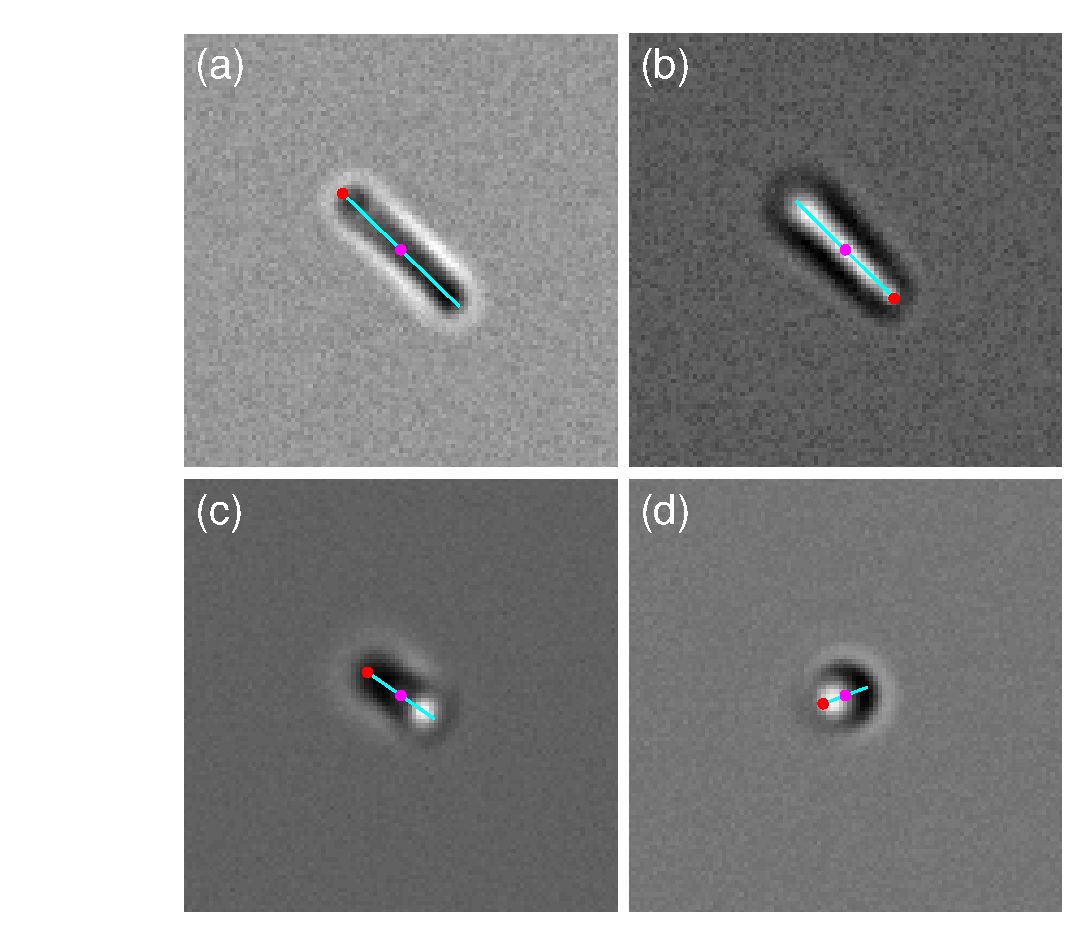
\includegraphics[scale=.4]{PolarRodTracking.eps}
\renewcommand{\baselinestretch}{1.0}
 \caption{ \small Typical appearances (or configurations) of a rod in optical images. Overlayed onto these images are the centroid (meganta dot), length and orientation (cyan line), and polarity of the rod (red dot) extracted from image analysis.} \label{fig:tracking}
%\end{center}
%\vspace{-1\baselineskip}
\end{figure}
The typical configurations and appearances of the particle are summarized in Figure SX (PolarRodTracking.eps), depending on the relative position of the body of the rod to the focal plane. We extract the centroid,  length, orientation, and the polarity (or the magnetic end) of the rod by a  Matlab-based script. Briefly, the background image ($im_b$) averaged over 1000 frames is first removed from the raw images ($im$) to obtain both positive ($im-im_b$) and negative ($im_b-im$) images, since a particle may have both dark and bright parts in the image. A bandpass filter is used to smooth and remove background noise [CrockerJCIS1996r; GaoOptEx2009] from the  images. These images are first analyzed separately and binarized by setting an intensity threshold, which is dynamically adjusted such that the smaller dimension of the bounding rectangle of the pixels above the threshold is within the average diameter of the rod ($0.65\pm 0.03 \mu m$, measured from SEM images of $\sim$ 70 particles) to mitigate the blurring effect from diffraction. The resulted bright and dark pixels above the threshold were then combined together. The orientation of the particle is determined by approximating these pixels by an ellipse through the ``regionprops'' function of Matlab, when the particle appears only dark or bright in the image; otherwise, the orientation is determined by the line linking the centroids of the dark and bright pixels [GaoOptEx2009]. The center and length of the particle is set as those of the bounding rectangle of the combined pixels. The last step is to track the polarity of the particle by tracking its ends. Minimization of the mean squared displacements of the two ends is used when the particle length ($L_p$) is above a threshold, while the appearances of the two ends (bright and dark for the ends above and below the focal plane respectively [CurtisOptComm2002; LeeOptEx2007.pdf]) is used when $L_p$ is below the threshold, since the appearances of the two ends will not change before $L_p$  going above the  threshold. The magnetic end appears slightly bigger and darker due to the presence of magnetite nanoparticles when the rod stays nearly flat on the coverslip, which is used to distinguish the two ends. Finally, we examine the quality of the image analysis and tracking by overlaying results to the images (Movie SI) and correct erroneous ones. 

\subsection*{\normalsize Enhanced entropic reorientation on particles of different sizes}
\begin{figure}[!ht]
%\setlength{\intextsep}{-20pt} \vspace{-.5\baselineskip}
\begin{center}
\includegraphics[scale=.45]{Ptheta-allFL.eps}
\renewcommand{\baselinestretch}{1.0}
 \caption{ \small Histograms of $\theta$ for 3 particles of different sizes with $Lp$ of 4.025, 3.5, 3.5 and 3.38 $\mu m$ without (blue circles) and with (red circles) applied magnetic field. Blue lines are fits to the experimental data at zero field according to equation xx. The red lines are predictions of the theory based on measured properties of the rod, with details listed in Table 1. } \label{fig:ptheta}
\end{center}
\vspace{-1\baselineskip}
\end{figure}
In Fig XX, we show resuts on three particles of different sizes. The histograms at zero field are fit to $ P(\theta)\sim \exp(-a\cos \theta )\sin \theta $ to extract $a$, the gravitational energy of the rod when it stands vertically, with results listed in Table 1.  
The magnetic trap stiffness of each particle is calculated based equalpartition theorem by measuring the fluctuation of $\phi$ when the rod stays flat in the imaging plane, which we can measure in high accuracy. 

The average diameter and length of the rods  are $0.65 \pm 0.03 \mu m$ and $3.5 \pm 0.2 \mu m$, respectively, measured from $\sim 70$ rods from SEM images. 



\begin{center}
\centering
\begin{tabular}{|c|c|c|c|}
\hline
Particle ID & 1 & 2 & 3\\
\hline
L ($\mu m$)  &  4.025 &  3.5 & 3.38\\
\hline
a ($k_BT$) & 4.8$\pm$0.9 & 3$\pm$0.4 & 1.7$\pm$0.4\\
\hline
$\mu B (k_BT)$ & 168 & 150 & 180 \\
\hline
$\mu $  (remove it?)& 1.68 & 1.07 & 1.29 \\
\hline
\end{tabular}
\end{center}

Reply to Andrew's comments or questions:\\
1: I didn't include 'gimbal lock' in the title. Not sure if it sounds right, plus I'm not even sure its a strong enough argument to be the real selling point\\
1R:\\
2. The intro still needs some work, it's the bit I'm least satisfied with so far\\
R:\\
3. Is the rod a nanorod? A comment from my poster session at Boulder was that something 0.65 x 3 µm isn't really 'nano' as its more 'micro'\\
R: Agree. Change it to microrod. \\
4. Is there a reference for the synthesis yet? Or a preprint i can reference?\\
R: We should add in the reference of  Kuijk et al JACS. What about our own synthesis paper?\\
5. Should the image analysis technique be included too or should that go in the SI?\\
R: Yes, put it in the SI.\\
6. How long did the experiments run for? 60 minutes? or were they different lengths\\
R: 10 and 20 minutes for without and with field respectively.\\ 
8. I removed the theory heat map from underneath the scatter plot. I didn't think it was adding much that isn't shown elsewhere.\\
R: Not sure, I kind of like how it looks. You can decide on this.\\
9. I kept in (but reduced and streamlined) the maths at the end. I still think its important to include as an explanation for why we shouldn't expect the probability -ln(P) to be an energy landscape. The fundamental reason why its not is because the angles are all coupled to each other in the potential energy.\\
R: I am open to it.


Other comments:\\
(1) Change discussion from magnetic field strength (B) to the magnetic potential or magnetic trap stiffness ($\mu B$) since what matters is the product of $\mu$ and B. \\
(2) We have done experiments on multiple particles, whose gravitational potential seems to vary quite a bit. It appears to me now it is more appropriate to extract the gravitational potential from the fit to data without applied field.  
(3) Make it clear that the 'bistability' refers to Figure 4 (a) and (b). 



\end{document}
